\documentclass[../../main.tex]{subfiles}
\begin{document}
\begin{center}
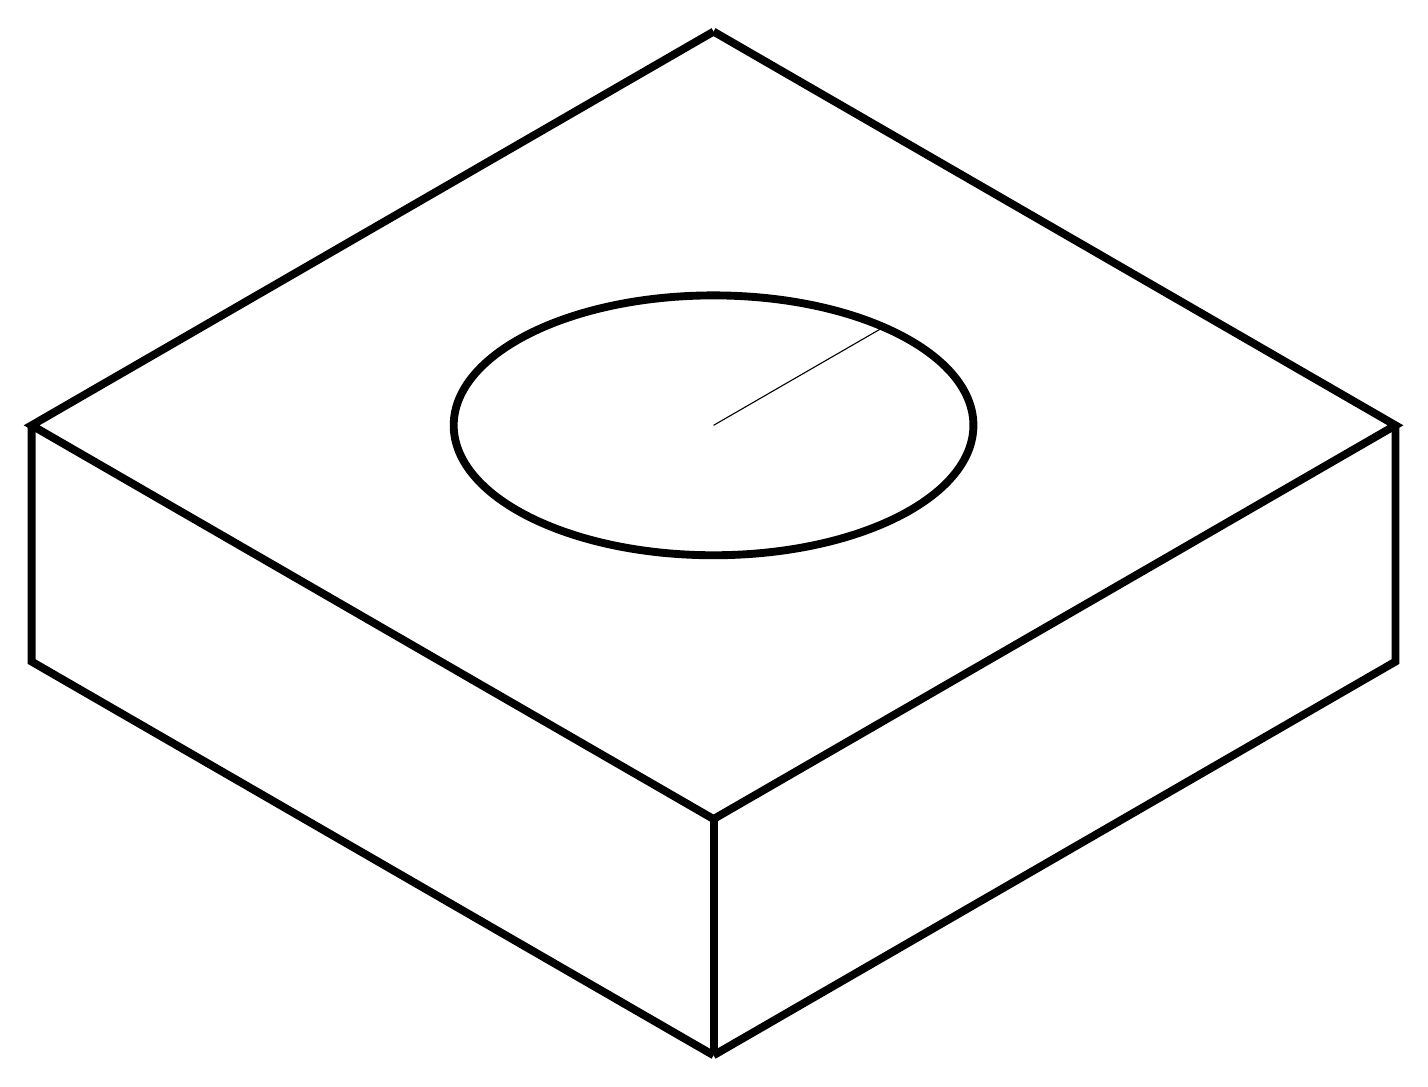
\begin{tikzpicture}[scale=0.1,font=\sffamily]
\draw [line width=1mm](0,0)--(0,30);
\draw [line width=1mm](0,0)--(30:100)--++(0,30);
\draw [line width=1mm](0,0)--(150:100)--++(0,30);
\draw [line width=1mm](0,30)--++(150:100)--++(30:100);
\draw [line width=1mm](0,30)--++(30:100)--++(150:100);
\draw [line width=1mm](0,30+50) ellipse (33 and 16.5);

\draw (0,80)--++(30:25);


\end{tikzpicture}
\end{center}
\end{document}